\documentclass[12pt,fleqn]{article}
\usepackage{
  amsmath,
  booktabs,
  geometry,
  graphicx,
  microtype,
  parskip,
}
\usepackage[shortlabels]{enumitem}

\geometry{margin=3cm}

% equation line spacing
\setlength{\jot}{0.5cm}

% meta data
\newcommand{\chapter}{3.3}
\newcommand{\authorname}{Amo DelBello}
\newcommand{\classdescription}{MATH 1350-D2}
\newcommand{\classname}{Introduction to Statistics, Fall 2022}
\newcommand{\assignment}{\chapter\ Book Assignment}

\newcommand{\problem}[1]{\vspace{5ex}\section*{\chapter-#1}}
\newcommand{\thead}[1]{\textnormal{\textbf{#1}}}
\newcommand{\tvspace}{\vspace{.25cm}}

\title{\classdescription\ \\ \classname\ \\ $\ $ \\ \assignment}
\author{\authorname}
\date{\today}


\begin{document}
\maketitle

\problem{5}
\begin{enumerate}[(a)]
  \item The difference between Verizon's data speed at ATL and the mean of all Verizon's data speeds is $77.8 - 17.60 = 60.2~\text{Mbps}$
  \item $\frac{60.2}{16.02} = 3.76$ standard deviations
  \item $z = \frac{x - \bar{x}}{s} = \frac{77.8 - 17.60}{16.02} = 3.76$
  \item Yes. Verizon's data speed at ATL is significantly high because its z score (3.76) is greater than 2.
\end{enumerate}

\problem{8}
\begin{enumerate}[(a)]
  \item The difference between the weight of 5.28 lb and the mean of the weights is $5.28 - 1.911 = 3.369~\text{lb}$
  \item $\frac{3.369}{1.065} = 3.16$ standard deviations
  \item $z = \frac{x - \bar{x}}{s} = \frac{5.28 - 1.911}{1.065} = 3.16$
  \item Yes. The weight (5.28 lb) is significantly high because its z score (3.16) is greater than 2.
\end{enumerate}


\problem{11}
The coins that are significantly high or low are those with a weight of $5.63930 \pm 2(0.06194)$, that is: $> 5.76318$ or $< 5.51542$.


\problem{15}
\begin{equation*}
  z = \frac{x - \bar{x}}{s}
\end{equation*}
\textbf{Male:} $\frac{1500 - 3272.8}{660.2} = -2.69$

\textbf{Female:} $\frac{1500 - 3037.1}{706.3} = -2.18$

The male has the weight that is more extreme relative to the group from which they came with a z score of $-2.68$.


\problem{17}
\begin{equation*}
  \text{Percentile value of } 2.4~\text{Mbps} = \frac{29}{50} * 100 = 58
\end{equation*}


\problem{18}
\begin{equation*}
  \text{Percentile value of } 13.0~\text{Mbps} = \frac{45}{50} * 100 = 90
\end{equation*}


\problem{21}
\begin{align*}
  L &= \frac{k}{100}n \\
  L &= \frac{60}{100}(50) = 30
\end{align*}
30 is a whole number so $P_{60} = (2.4 + 2.5) / 2 = 2.45~\text{Mbps}$


\problem{24}
\begin{align*}
  L &= \frac{k}{100}n \\
  L &= \frac{40}{100}(50) = 20
\end{align*}
20 is a whole number so $P_{40} = (1.0 + 1.1) / 2 = 1.05~\text{Mbps}$


\problem{30}
\begin{align*}
  \text{min} &= 0.51 \\
  \text{max} &= 1.49
\end{align*}

\begin{align*}
  Q_{25} &= P_{25} \\
  L &= \frac{25}{100}(11) = 2.75 \\
  L &= 3~ \text{rounded up} \\
  Q_{25} &= 0.89
\end{align*}

\begin{align*}
  Q_{50} &= P_{50} \\
  L &= \frac{50}{100}(11) = 5.5 \\
  L &= 6~ \text{rounded up} \\
  Q_{50} &= 1.38
\end{align*}

\begin{align*}
  Q_{75} &= P_{75} \\
  L &= \frac{75}{100}(11) = 8.25 \\
  L &= 9~ \text{rounded up} \\
  Q_{75} &= 1.45
\end{align*}

\begin{figure}[ht]
  \centering
  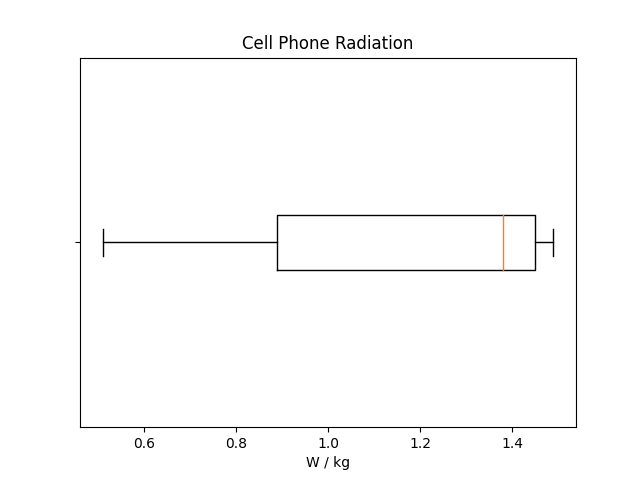
\includegraphics[width=12cm]{assets/cell-phone-radiation.png}
  \caption{Cell Phone Radiation}
\end{figure}


\pagebreak
\problem{33}
\begin{figure}[ht]
  \centering
  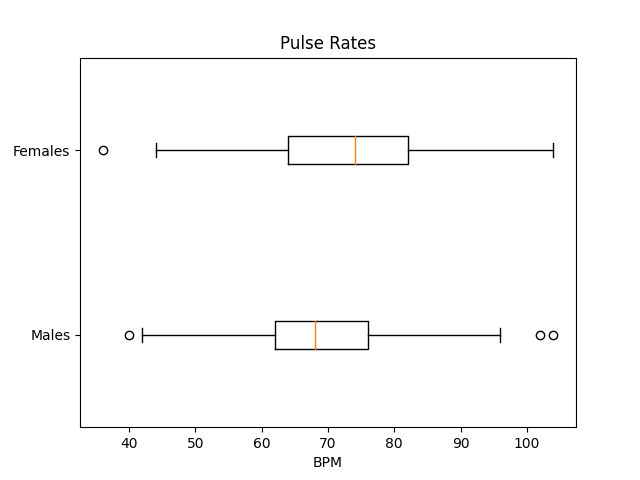
\includegraphics[width=12cm]{assets/pulse-rates.png}
  \caption{Male \& Female Pulse Rates}
\end{figure}
On average, females appear to have slightly higher pulse rates.

\end{document}
%%% Local Variables:
%%% mode: latex
%%% TeX-master: t
%%% End:
